
\documentclass{article}

\usepackage[ngerman]{babel}                     %for german umlauts
\usepackage[utf8]{inputenc}
\usepackage{subfigure}
\usepackage{float}
%\usepackage[framed,autolinebreaks,useliterate]{mcode}
%\usepackage[bw,framed,autolinebreaks,useliterate]{mcode}
% \usepackage[ansinew]{inputenc}        %for german umlauts

\usepackage{listings}

\usepackage{graphicx}
\usepackage{hyperref}

\usepackage{amssymb}    %for different fonts
\usepackage{amsmath}
% Geht nicht: \usepackage{bbm}
% \usepackage[usenames,dvips]{color} %only way to get it running with pdf:(
% \usepackage[pdftex,usenames,dvipsnames]{color}        % does not work
% \usepackage{color}
\usepackage{verbatim}
\usepackage{polynom}

\usepackage{tikz}
\usetikzlibrary{trees,shapes,snakes}

\setlength{\parindent}{0pt}
\addtolength{\hoffset}{-2cm}
\addtolength{\voffset}{-1cm}
\addtolength{\textheight}{3cm}
\addtolength{\textwidth}{3cm}

\newcommand{\im}{\operatorname{Im}}
\newcommand{\rg}{\operatorname{rg}}
\newcommand{\ggt}{\operatorname{ggT}}

\lstset{ %
  language=Matlab,                % the language of the code
  frame=single,                   % adds a frame around the code
  tabsize=2,
  basicstyle=\footnotesize
}

\begin{document}

\section*{\begin{center} Mustererkennung - Aufgabenblatt 12 \end{center}}
\begin{center}
  André Hacker und Dimitri Schachmann \\
\end{center}


\subsection*{1. WEKA}
In dieser Aufgabe haben wir uns das WEKA Framework angeschaut und ausprobiert in
den folgenden Screenshots sieht man, wie wir die wildfire Daten geladen und
klassifiziert haben.\\[2em]
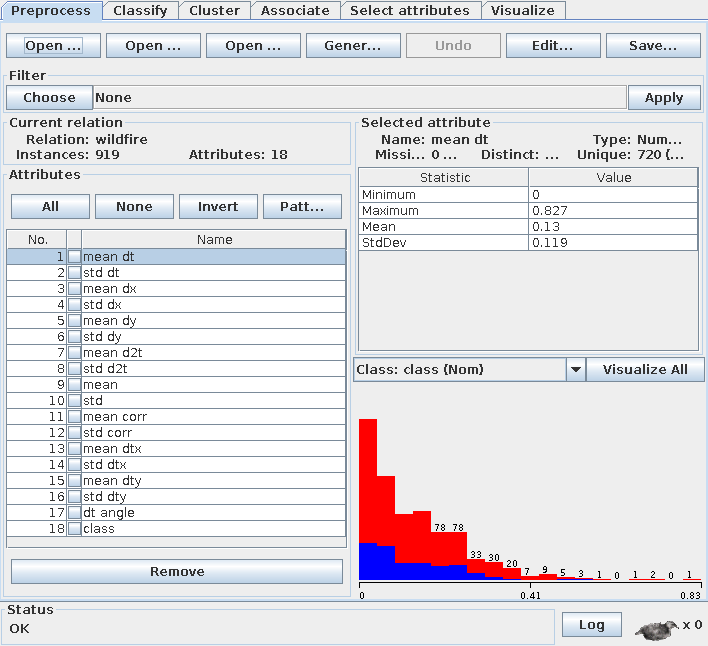
\includegraphics[scale=0.6]{WEKA1.png}\\[2em]
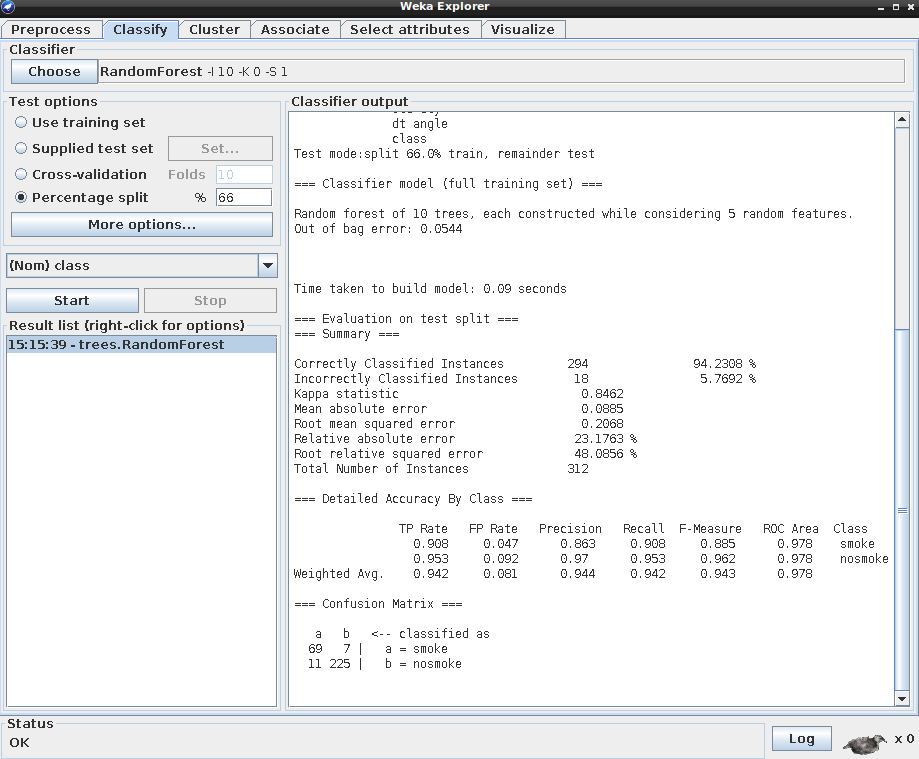
\includegraphics[scale=0.5]{WEKA2.png}\\[2em]
Man sieht, dass die Klassifikation sehr gut ist und auch schnell von statten
geht.\\

K-fold Classification haben wir uns angesehen und getestet - eine sehr einfache und intuitive Methode.\\

Sehr praktisch sind auch die Histogramme für die Werte der Features, über die man schnell einen Eindruck der Wertebereiche erhält. Außerdem wird angezeigt, welche Klasse bei welchem Wert des Features wie oft vorkommt, was etwas über die Korrelation des Features mit der Target-variable aussagt.\\

Wir sind sehr beeindruckt von diesem Framework.\\

\subsection*{2. Random Forests}

\subsubsection*{Hinweise zur Implementierung}
Wir machen zuerst einen Split der Daten in Test- und Trainingsdaten (aktuell $0.7$).\\
Die Bootstrap samples werden aus den Trainingsdaten zufällig gewählt (mit zurücklegen). Auf dieser Basis wird der Wald trainiert.\\

Wir verwenden den regulären Fischer Klassifikator in jedem Knoten. Zur Klassifizierung verwenden wir die maximale Wahrscheinlichkeit. Wir haben überlegt den Gini-Index für einen guten Threshold auf der Fisher-Diskriminante zu wählen, allerdings kam uns das etwas abenteuerlich vor, weil dies kein in der Litaratur erwähnter Weg ist. Wir haben daher zuerst den Standardweg implementiert und sind mit den Erkennungsraten (bis zu $0.96$) sehr zufrieden.\\

Wir berechnen den in-sample-error (bzw. die Erfolgsrate auf den Daten mit denen trainiert wurde) für jeden Baum sowie den out-of-sample error für den gesamten Wald auf Basis der vorher zurückgelegten Testdaten. Wie erwartet ist der in-sample-error deutlich besser, bei wenigen Daten bis zu 0 (da ja quasi auswendig gelernt wurde).\\

Die Funktion compute-node (siehe im Code-Anhang) macht deutlich, was in jeder Node gespeichert wird: Erstens die Modell-Parameter, also hier die Fisher Diskriminante und die Parameter der Verteilung. Und zweitens die Menge der zufällig ausgewählten Features.\\

Die folgende Funktion implementiert das Training und dokumentiert die Parameter unseres Modelles:

\begin{lstlisting}
% Trains a random forest given a training set X,Y
% @param M: number of bootstrap samples
% @param m: dimension for random subspace selection
% @param max_depth: limit for maximum depth, to avoid stack problems
% @return trees: The trained forest
% @return in_sample_success: Success-rate for the data we trained
%  on (for every tree separatly)
% @return depths: vector with the depths of all trained trees
function [trees, in_sample_success, depths] = ...
        random_forest_train(M, m, X, Y, max_depth, bootstrap_split)
    
    N = size(X,1);
    Nb = ceil(bootstrap_split*N);   % size of bootstrap sample

    in_sample_success = zeros(M,1);
    out_of_sample_success = zeros(M,1);
    trees = cell(M,1);
    depths = zeros(M,1);
    for i=1:M
        disp(['Train tree ' num2str(i)]);
        % Take bootstrap sample, i.e. draw with replacement
        bootstrap_indecies = randi(size(X,1),1,Nb);
        bootX = X(bootstrap_indecies,:);
        bootY = Y(bootstrap_indecies,:);
    
        [trees{i} depths(i)] = compute_subtree(bootX, bootY, m, 0, ...
                                           max_depth);
    
        %disp(trees{i}.tostring)

        % In-sample-error
        %in_sample_success(i) = checkError({trees{i}}, bootX, bootY);
        %out_of_sample_success(i) = checkError({trees{i}}, tesX, tesY);
    end

    disp('Trained forest:');
    disp(['M:' num2str(M) ' m:' num2str(m) ' N:' num2str(N) [' max-' ...
                        'depth:'] num2str(max_depth)]); 
    disp(['bootstrap-split:' num2str(bootstrap_split)  ...
          'bootstrap-sample-size:' num2str(Nb)]);

end

\end{lstlisting}

Wir haben folgende Implementierung der Baumstruktur verwendet:
http://www.mathworks.com/matlabcentral/fileexchange/35623-tree-data-structure-as-a-matlab-class\\

Folgende Beobachtungen haben wir gemacht:
\begin{itemize}
\item Für die Berechnung der optimalen Fisher muss die Inverse der Summe der Kovarianzmatrizen berechnet werden. In den unteren Knoten des Baumes sind aber häufig nur wenige Datensätze zu klassifizieren, z.B. 1 smoke und 2 non-smoke, so dass die Matrix keinen vollen Rang hat und nicht invertierbar ist. Wir haben das Problem gelöst, indem wir die Datensätze für die Berechnung der Kovarianzmatrix vervielfachen, mit leichtem Rauschen. Es verhält sich also so, als wären tatsächlich mehr Punkte an ähnlichen Stellen vorhanden. Dies hat das Problem und die mittlere Tiefe der Bäume deutlich reduziert (sichtbar bei kleineren Bäumen)
\end{itemize}

\subsubsection*{Ergebnisse}

Optimale Ergebnisse haben wir nicht wie erwartet mit $m=3$ sondern mit $m=2$ und $M=20$ erzielt. Die guten Ergebnisse waren reproduzierbar.\\
Im folgenden ein Auszug aus dem Log unserer Tests:

\begin{verbatim}
Nb = size of bootstrap samples
testSize = size of test sample (for out-of-sample error)
M = number of trees
m = dimensions
total_success = out-of-sample error for the forest

M=30 m=5
Nb = 516
testSize =183
total_success = 0.9180

M = 10 m = 5
Nb = 451
testSize = 275
total_success = 0.9200

M = 10 m = 5
Nb =451
testSize = 275
total_success = 0.8873

M = 20 m = 5
Nb = 580
testSize = 275
total_success = 0.9273

M = 20 m = 5
Nb =580
testSize = 275
total_success =0.9127

M = 50 m = 5
Nb = 580
testSize =  275
total_success =0.8909

M = 20 m = 2
Nb = 580
testSize = 275
total_success = 0.9673

M = 20 m = 2
Nb = 580
testSize = 275
total_success = 0.9491

M = 20 m = 3
Nb = 580
testSize =275
total_success =  0.9345

M = 5 m =2
Nb =580
testSize =275
total_success = 0.9236
\end{verbatim}

Ein Grund für die Wahl des Tree-Frameworks war die gute Visualisierung. So konnten wir zu Beginn kleinere Bäume visualisieren. Wie z.B. diesen hier:
\begin{lstlisting}
Trained forest:
M:1 m:2
N:644
bootstrap-split:0.01
bootstrap-sample-size:7

            <6x1 cell>
      +---------+-------+
      |                 |
 <6x1 cell>        <6x1 cell>
   +--+---+             |
   |      |             |
   1     -1        <6x1 cell>
                    +--+-------+
                    |          |
               <6x1 cell>     -1
                 +--+---+
                 |      |
                 1     -1
\end{lstlisting}

\subsubsection*{Code}
Hier der restliche Code:
\begin{lstlisting}
function r = rf()

    addpath('.')
    raw_data = csvread('wf.csv');
    X = raw_data(:,1:(end-1)); % the samples
    Y = raw_data(:,end);       % the labels

    % Split data. Always use same test data.
    split = 0.7;
    tra_size = ceil(split*size(X,1));

    rand_indecies = randperm(size(X,1));
    traX = X(rand_indecies(1:tra_size),:);
    traY = Y(rand_indecies(1:tra_size),:);
    tesX = X(rand_indecies(tra_size+1:end),:);
    tesY = Y(rand_indecies(tra_size+1:end),:);
    N = size(traX,1);

    m = 2;             % Number of features to use in each node
    max_depth = 1000;   % Just to avoid that we run out of stack
                       % memory! Usually we would not limitate the depth
    set(0, 'RecursionLimit', 10000);
    M = 5;              % Number of trees
    bootstrap_split = 0.9;
    
    [trees, in_sample_success, depths] = ...
        random_forest_train(M, m, traX, traY, max_depth, bootstrap_split);

    %in_sample_success
    %out_of_sample_success
    
    % Test out of sample error
    total_success = checkError(trees, tesX, tesY)
    meanDepth = mean(depths)
    testSize = size(tesY,1)
end

% Compute forest success rate
function success_rate = checkError(trees, X, Y)
    N = size(X,1);
    M = size(trees,1);
    predictions = zeros(N,M);
    for j = 1:M
        for i = 1:N
            predictions(i,j) = predict_tree(trees{j}, X(i,:), Y(i,:));
        end
        disp(['predicted for tree ' num2str(j)]);
    end
    prediction = mode(predictions,2);
    
    success_rate = sum([prediction==Y])/N;
end

% Predict output for single input x using tree t
function prediction = predict_tree(t, x, y)
    id = 1;
    while true
        if t.isleaf(id)
            found = true;
            % Get predicted class
            prediction = t.get(id);
            return
        end
        % Get discriminant and threshold
        content = t.get(id);
        features = content{1};
        fisher_disc = content{2};
        mu0 = content{3};
        mu1 = content{4};
        s0 = content{5};
        s1 = content{6};
        
        % Take subset of features
        xsub = x(1, features);
        prediction = fisher_predict(xsub, fisher_disc, mu0, mu1, s0, ...
                                    s1);
        % Go left or right, depending on result
        childids = t.getchildren(id);
        if size(childids)==1
            % We could have skipped prediction, go down!
            id = childids(1);
        else
            if prediction == 1
                % Go left
                id = childids(1);
            else
                % Go right
                id = childids(2);
            end
        end
    end  % while true
end

% Predicts class for a single value x
function prediction = fisher_predict(x, disc, mu0, mu1, s0, s1)
    % test with test data
    projection = project(x, disc);
     % compute the propabilties for each test sample and the two classes.
    P = [gaussDensity(mu0, s0, projection) ...
         gaussDensity(mu1, s1, projection) ];
    [maxValue maxIndex] = max(P,[],2);
    
    % contains the predicted classes
    classes = [1 -1];
    prediction = classes(maxIndex);    
end


% Recursively called function creating the tree
function [subtree real_depth] = compute_subtree(traX, traY, m, current_depth, max_depth)

    %disp(['depth ' num2str(current_depth)]);
    real_depth = current_depth;
    % Anchor: Check if all are from same class
    if (all(traY == traY(1,1)))
      subtree = tree(traY(1,1));
      return
    end

    % To be removed, we let it grow until data are separated
    if (current_depth >= max_depth && max_depth > 0)
      subtree = tree(mode(traY));
      return
    end
    
    [node prediction] = compute_node(traX,traY,m, current_depth);
    
    subset_pos_X = traX(prediction==1,:);
    subset_pos_Y = traY(prediction==1);
    subset_neg_X = traX(prediction==-1,:);
    subset_neg_Y = traY(prediction==-1);

    subtree = tree(node);
    
    % Recursive call to create both subnodes
    if (size(subset_pos_X,1)>0)
      [subtree_pos depth_left] = compute_subtree(subset_pos_X,subset_pos_Y,m,current_depth+1,max_depth);
      subtree = subtree.graft(1,subtree_pos);
      real_depth = depth_left;
    end
    if (size(subset_neg_X,1)>0)
      [subtree_neg depth_right] = compute_subtree(subset_neg_X,subset_neg_Y,m,current_depth+1,max_depth);
      subtree = subtree.graft(1,subtree_neg);
      real_depth = max(real_depth,depth_right);
    end

end


% @return node: cell containing:
%  1) Model parameters: Here Fisher discriminant a (to project on)
%     and distribution parameters (mean and std-dev of both classes)
%  2) Features: The randomly selected subset of features (indices)
% @return prediction: column vector with predicted classes for all
%  training items
function [node prediction] = compute_node(traX, traY, m, current_depth)
    feature_indecies = randperm(size(traX,2));

    current_data = traX(:,feature_indecies(1:m));
    current_y = traY;

    % TODO: IF THERE ARE NOT ENOUGH DATA, COPY DATA/MAKE SOME NOISE!
    tra_pos = filterByClass(current_data, current_y,1);
    tra_neg = filterByClass(current_data, current_y,-1);
    
    mu0 = mean(tra_pos,1);
    sigma0 = cov(tra_pos);
    mu1 = mean(tra_neg,1);
    sigma1 = cov(tra_neg);
    
    % COMPUTE FISHER DISCRIMINANT
    covSum = sigma0 + sigma1;
    if (rank(covSum) < size(covSum,1))
        % Not invertible. Take every sample multiple times with
        % slightly modification
        %disp(['depth' num2str(current_depth) ' Not invertible -> make some noise!']);
        posCount = size(tra_pos,1);
        negCount = size(tra_neg,1);
        tra_pos_tmp = tra_pos;
        tra_neg_tmp = tra_neg;
        for i=1:3
           tra_pos_tmp = [tra_pos_tmp; tra_pos+rand(posCount,m)*0.01];
           tra_neg_tmp = [tra_neg_tmp; tra_neg+rand(negCount,m)*0.01];
        end
        posCountAfter = size(tra_pos_tmp,1);
        negCountAfter = size(tra_neg_tmp,1);
        % Recompute covariances
        sigma0 = cov(tra_pos_tmp);
        sigma1 = cov(tra_neg_tmp);
        covSum = sigma0 + sigma1;
        % Bad workaround:
        %covSum = covSum + eye(size(covSum,1))*0.001;
    end
    a = (mu0 - mu1) / covSum;   % error if covSum is not invertible
    a = a / norm(a);

    % PROJECTION to 1d normal distribution
    psigma0 = a * sigma0 * a';
    psigma1 = a * sigma1 * a';    
    pmu0 = project(mu0, a);
    pmu1 = project(mu1, a);
  
    % CLASSIFY CURRENT SUBSET
    projection = project(current_data, a);
     % compute the propabilties for each test sample and the two classes.
    P = [gaussDensity(pmu0, psigma0, projection) ...
         gaussDensity(pmu1, psigma1, projection) ];
    [maxValue maxIndex] = max(P,[],2);
    
    % contains the predicted classes
    classes = [1 -1];
    prediction = classes(maxIndex)';
    
    node = { feature_indecies(1:m)
             a
             pmu0
             pmu1
             psigma0
             psigma1};
    
    %success_rate = sum([prediction==current_y])/size(current_data,1)
end


function r = filterByClass(samples, labels, c)
  r = samples(ismember(labels,c),:);
end



function p = project(x, a)
  if (size(x,1)>1)
    p = dot(x, repmat(a, size(x,1),1), 2);
  else
    p = dot(x,a);
  end
end


function p = gaussDensity(mu, sigma, data)
  normalize = 1 / (sqrt(2*pi) * sigma);
  p = zeros(size(data,1), 1);
  for i=1:size(data,1)
    p(i) = normalize * exp( -(data(i)-mu)^2 / (sigma^2) );
  end
end
\end{lstlisting}



\end{document}
